\documentclass{article}
\usepackage[a4paper,top=2cm,bottom=2cm,left=2cm,right=2cm]{geometry}
\usepackage[english]{babel}
\usepackage[T1]{fontenc}
\usepackage[utf8]{inputenc}
\usepackage{fancyhdr}
\usepackage{float}
\usepackage{graphicx}
\usepackage{wrapfig}
\usepackage{siunitx} %per scrivere il simbolo °
\usepackage{verbatim} %per i commenti1
\usepackage{amsmath}
\usepackage[linesnumbered, ruled, vlined]{algorithm2e}
\setcounter{secnumdepth}{3}
\setcounter{tocdepth}{6}
\usepackage{multirow}
\newcommand{\minitab}[2][l]{\begin{tabular}#1 #2\end{tabular}}
\usepackage{rotating}
\usepackage{xfrac}
\usepackage{cite}
\usepackage{caption}
\usepackage{subcaption}

\DeclareMathOperator*{\argmax}{arg\,max}
\DeclareMathOperator*{\argmin}{arg\,min}

%\usepackage{booktabs,array}
%\usepackage{tikz}

%\usepackage{tabularx}

%\usepackage{chngcntr}
%\counterwithin{table}{section}

%------------------------------ colors
\usepackage[usenames,dvipsnames,table]{xcolor} % use colors on table and more
\definecolor{333}{RGB}{51, 51, 51} % define custom color
\definecolor{background}{RGB}{248, 248, 255}
\definecolor{comment}{RGB}{17,167,5}
\definecolor{keyword}{RGB}{195,47,8}
\definecolor{string}{RGB}{142,195,0}
\definecolor{number}{RGB}{90,84,84}
\definecolor{identifier}{RGB}{0,90,201}

%------------------------------ source code
\usepackage{listings}

\lstset{
  basicstyle=\footnotesize\sffamily,
  commentstyle=\itshape\color{gray},
  captionpos=b,
  frame=shadowbox,
  language=HTML,
  rulesepcolor=\color{333},
  tabsize=2
}

\title{\textbf{Report about Project}} % Title
\author{Raffaele \textsc{Di Nardo Di Maio} 1204879} % Author name
\date{\today}

\begin{document}
\begin{minipage}{.20\textwidth}
  
\includegraphics[height=3cm]{../Icon4}
\end{minipage}\begin{minipage}{.20\textwidth}
  \begin{table}[H]
  \begin{tabular}{l}
  \scshape{\Large{Computer Engineering Master Degree}} \\
  \hline \\
  \scshape{\Large{Computer Vision}} \\
  \end{tabular}
  \end{table}
\end{minipage}
{\let\newpage\relax\maketitle}

\section{Project details}\label{details}
The goal of the experience was to estimate in an image the best match from a series of views of an object that we are trying to localize. 
\begin{enumerate}
\item{\textbf{Computation of $\gamma$-transform}\\
this transform was applied to increase the contrast and stretch very high values in the images. In fact the values of the gamma values are all greater than 1. This transformation was applied only to views because of very strong brightness in them.}
\item{\textbf{Computation of Canny detection}\\
Canny detector is applied to test images and also to $\gamma$-transformed views.}
\item{\textbf{Matching phase}\\
this phase is performed using two different approaches, depending on specification of optional argument \texttt{-dist} (see Section \ref{args}). These approaches are:
\begin{itemize}
\item{\textbf{Template Matching with distance transform}\\
The distance transformed is applied to each test image and then the function \texttt{cv::matchTemplate()} is applied to the result of the transform using Canny detected view as template. The metric used is the \textit{Template Matching Correlation Coefficient (TM\_CCOEF} in opencv\textit{)}. Then I search the max value in the resulting matrix and using the position of that pixel as the position of the template for the match. With this approach I take only the ten best matches for each image, as specified in the assignment. The score value used to establish the best matches is the value contained in the max entry of result matrix.
}
\item{\textbf{Template Matching with histogram refinement}\\
The template matching is performed looking to TM\_CCOEF as in the previous approach on the test image with detected edges and using view image with detected edges as template. To improve the results obtained, I don't take only the 10 best matches but the 50 best results and then I apply a refinement algorithm based on histogram. For each previously computed match I compute a sub-window, related to the position of found match and with size equal to the related view, and I filter it with the corresponding mask. This RGB sub-window of the original test image is then converted to the HSV space and its histogram of the Hue channel is computed. The resulting histogram is then compared with the Hue histogram of the original view image using \texttt{cv::compareHist()}. The final score of a match is the following:
$$final\_score=\alpha*match\_score + \beta*hist\_score$$
where \textit{match\_score} is the score obtained by applying only \texttt{cv::matchTemplate()} and \textit{hist\_score} is the score obtained by \texttt{cv::compareHist()}. Hence from the set of 50 best matches only 10 best matches survive.}
\end{itemize}
}
\item{\textbf{Generation of result text files and result images}\\
for each mask of 10 best matches, its egdes are highlighted in red and printed in position evaluated before over the image (see Figure \ref{example_matching}). Each result image has a name with this format:
\begin{center}
\begin{tabular}{c}
\begin{lstlisting}[linewidth=120pt, basicstyle=\footnotesize\sffamily,]
datasetNum_matchNum.jpg
\end{lstlisting}
\end{tabular}
\end{center}
where \texttt{datasetNum} is the name of the dataset folder (it can be \textit{can}, \textit{driller} or \textit{duck}) followed by the number of the corresponding test image and \textbf{matchNum} is the number of the corresponding mask/view.
For each dataset the matches are written in the corresponding result text file with format specified in the assignment.}
\end{enumerate}
\begin{figure}[H]
\begin{subfigure}{.5\textwidth}
  \centering
  % include first image
  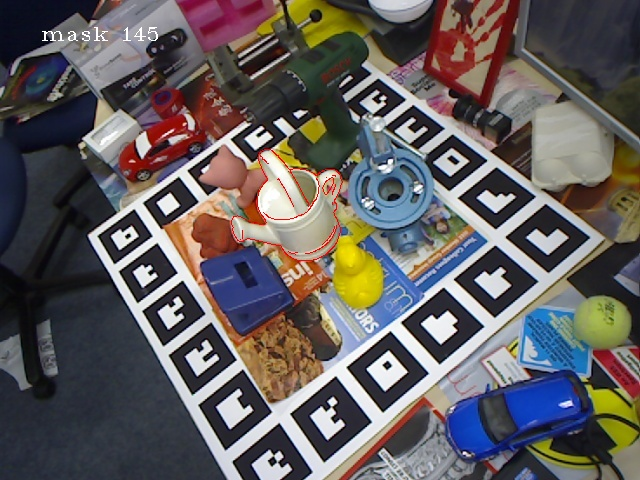
\includegraphics[width=.9\linewidth]{Images/can_dist.jpg}
  \caption{can0\_0.jpg}
\end{subfigure}
\begin{subfigure}{.5\textwidth}
  \centering
  % include second image
  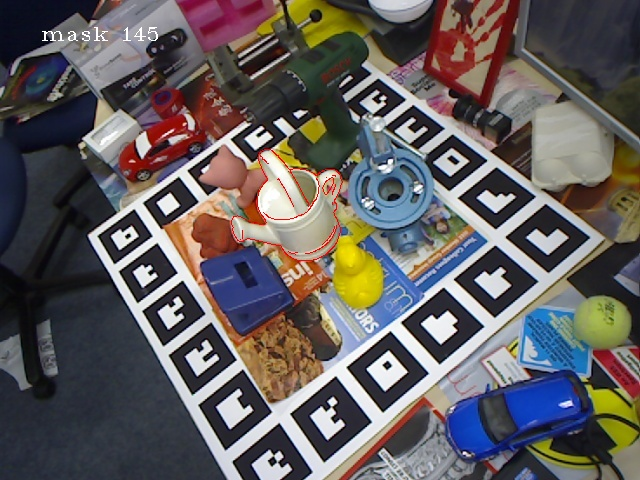
\includegraphics[width=.9\linewidth]{Images/can_refinement.jpg}  
  \caption{can0\_0.jpg}
\end{subfigure}
\newline
\begin{subfigure}{.5\textwidth}
  \centering
  % include third image
  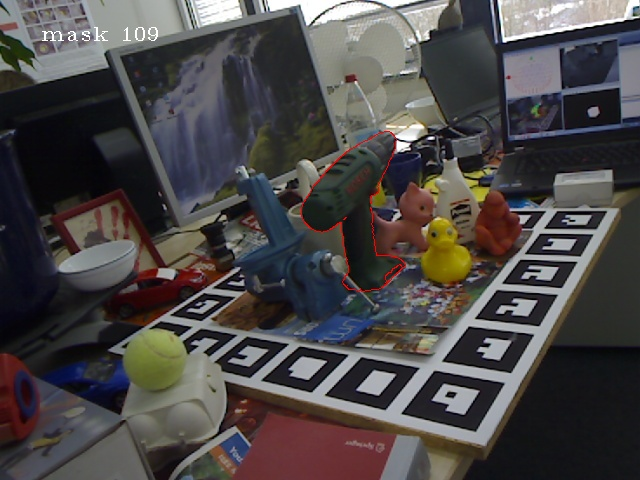
\includegraphics[width=.9\linewidth]{Images/driller_dist.jpg}  
  \caption{driller0\_0.jpg}
\end{subfigure}
\begin{subfigure}{.5\textwidth}
  \centering
  % include fourth image
  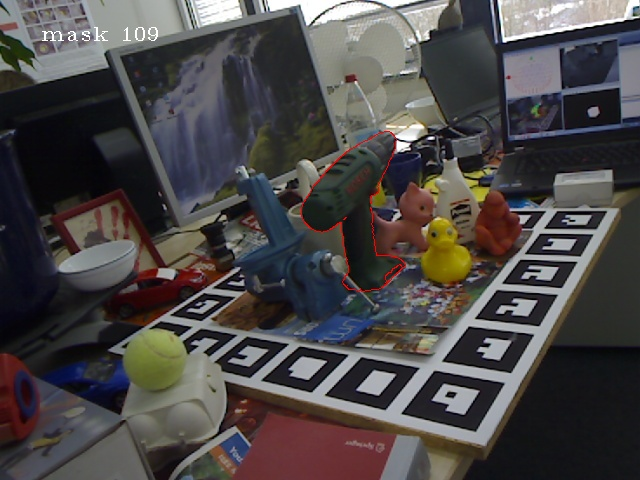
\includegraphics[width=.9\linewidth]{Images/driller_refinement.jpg}  
  \caption{driller0\_0.jpg}
\end{subfigure}
\newline
\vspace{0.5cm}
\begin{subfigure}{.5\textwidth}
  \centering
  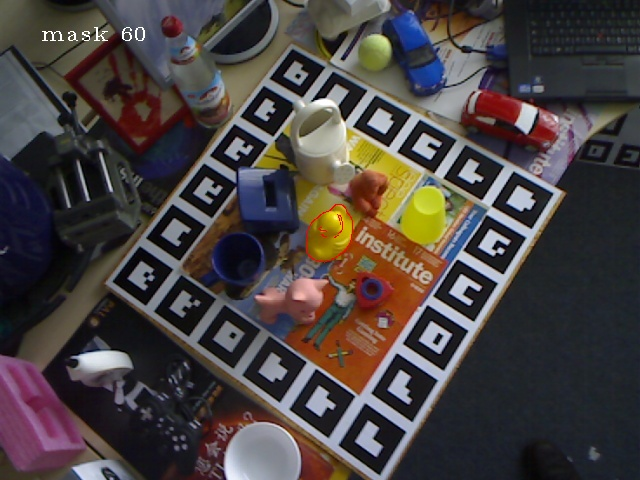
\includegraphics[width=.9\linewidth]{Images/duck_dist.jpg}  
  \caption{duck0\_0.jpg}
\end{subfigure}
\begin{subfigure}{.5\textwidth}
  \centering
  % include fourth image
  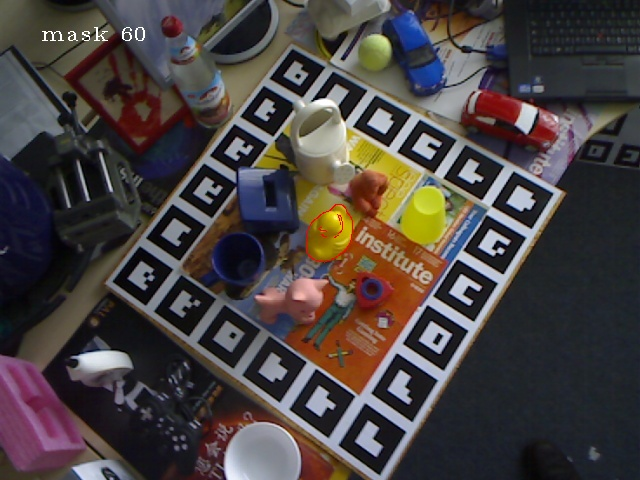
\includegraphics[width=.9\linewidth]{Images/duck_refinement.jpg}  
  \caption{duck0\_0.jpg}
\end{subfigure}
\caption{Example of result images with highlighted detected edges of views (left for Distance Transform approach, right for Histogram Refiniment approach).}
\label{example_matching}
\end{figure}

\subsection{Experimental results}\label{exp}
Looking to details of previous analysed steps of the implementation, I explain the reasons and the results obtained with the previous operations:
\begin{enumerate}
\item{\textbf{Computation of $\gamma$-transform}\\
The $\gamma$-transform was applied after different trials because of the precence of too many week edges and the colours of the views. Instead of using this transform, I tried also to equalize images before but the results were worst than obtained ones without any single-pixel operations. After different trials, the final values of $\gamma$ in $\gamma$-transform applied to each set of views are the following:
\begin{table}[H]
\footnotesize\centering
\begin{tabular}{rccc}
\cline{2-4}
& \textbf{can} & \textbf{driller} & \textbf{duck}\\
\hline
{$\mathtt{\gamma}$} & {1.4} & {1.3} & {1.4}\\
\hline
\end{tabular}
\caption{\footnotesize{$\gamma$ values for $\gamma$-transform applied on views of each dataset.}}
\end{table}
}
\item{\textbf{Computation of Canny detection}\\
For each dataset I defined two different high threshold of Canny detector for each dataset: the first for the views and the second for test images. Then looking to the results obtained, I assigned to low thresholds of Canny detector the value of the high thresholds decreased of a specific quantity: 30 for views and 40 for test images. The values for high thresholds are the following:
\begin{table}[H]
\footnotesize\centering
\begin{tabular}{rccc}
\cline{2-4}
& \textbf{can} & \textbf{driller} & \textbf{duck}\\
\hline
\textbf{test images} & {150.0} & {150.0} & {100.0}\\
\hline
\textbf{views} & {100.0} & {160.0} & {100.0}\\
\hline
\end{tabular}
\caption{\footnotesize{High thresholds for Canny detector.}}
\end{table}
The values of high thresholds are both smaller than other ones for \textit{duck} dataset because of need of more details for detection of shape of wing and beak.
}
\item{\textbf{Matching phase}\\
In this phase for each image of each dataset, the two methods obtain both all the best feasible matches. For both approaches, the matching was more simple on \textbf{can} dataset and very complex for several images of \textbf{driller} and \textbf{duck} datasets. In particular the method with distance transform is more efficient in terms of memory occupation because it stores less results.
In many images the histogram refinement approach obtains best results with wrong matches, positioning matches around the zone of the object to search even if they have a little bit wrong shapes.\\
The main problem of first method based on histogram refinement was to find the best thresholds for Canny detection for \texttt{driller} and \texttt{duck} because of some problems based on the shapes. In particular for \texttt{driller} matching, too small values for high Canny threshold help me to identify better the object in some images but loosing the correct matches on other ones. The same happens with too big values for high Canny threshold.\\
The reason comes from the level of contrast of different images and the smoothness of someone, that was very highlighted in several \textbf{can} images. The histogram comparison was performed only on Hue channel because of difference saturation and value of test image object and the corresponding model. For the same reason, to enhance the accuracy of comparison I did not work in RGB colour space. I tried another approach to estimate final score from histogram comparison without combining it with the previous one. I try to use only the histogram comparison score to discover from the set of 50 best matches the new 10 best ones. I used two approaches: 
\begin{itemize}
\item{Take only matches with the score of histogram comparison greater than a specified threshold}
\item{Take the 10 matches with highest score of histogram comparison}
\end{itemize}
For both methods, I notice that having higher scores of histogram comparison doesn't mean that there will not be false positive. In fact there were a lot of wrong matches and for this reason I decide to give an higher weight to previous Template Matching score and combine them in the following final score:
$$final\_score=100*match\_score + hist\_score$$}
\end{enumerate}
\section{Code}
\subsection{Performance}
The program can run analysing only one dataset or all the datasets in parallel. The management of this behaviour was done by using threads. Each thread performs the template matching on a dataset and the terminal window, for log printing, is the only resource managed using mutual exclusion.\\
Referencing to Section \ref{details}, I'm going to discuss the little tricks that I used to improved efficiency of the phases of the algorithm:
\begin{enumerate}
\item{\textbf{Computation of $\gamma$-transform}\\
To reduce the number of computation performed by the gamma transform, I compute only once, at the creation of the object related to Gamma Transform, a vector of size equal to the number of levels that has in position \textit{i} the value of the $\gamma$-transform for the input \textit{i}.}
\item{\textbf{Computation of Canny detection}\\
The computation of Canny detection for each view image is performed before the Matching phase and the results are stored. In this way then we need to compute the edges only once for each test image.
}
\item{\textbf{Matching phase}\\
To improve the efficiency of the buffer containing the best matches for each image of each dataset, I use a sorted vector (sorted by increasing score of matching) and I insert every element without loosing the sort. Every time that I obtain the best position/score of a mask in the template matching, I try to insert it in the best results buffer following this approach:\\\\
\begin{minipage}{.999\linewidth}
\begin{algorithm}[H]
\DontPrintSemicolon
\BlankLine
  \If{$\mathtt{buffer}\;is\;full$}{
    \BlankLine
	\If{$\mathtt{match}.score < \;\mathtt{buffer[0]}.score$}{
	  	$buffer.insert\_ordered(element)$
	}
    \BlankLine
  }
  \Else{
  	$\mathtt{buffer.}insert\_ordered(\mathtt{element})$
  }
  \BlankLine
  \caption{\textbf{Insertion}}
\end{algorithm}
\end{minipage}
\vspace{0.5 cm}
\\The insertion is based on the search of the position in the buffer for which the new match has a score that maintains sorted the vector. The manage of best matches for the created methods is done in the following way:
\begin{itemize}
\item{\textbf{Template Matching with distance transform}\\
for each test image a buffer of max size equal to 10 is created. In the first buffer the best match of each view is inserted in the buffer with score obtained by \texttt{cv::matchTemplate()}.
}
\item{\textbf{Template Matching with histogram refinement}\\
for each test image a buffer of max size equal to 50 and then a buffer of max size equal to 10 are created. In the first buffer the best match of each view is inserted in the buffer with score obtained by \texttt{cv::matchTemplate()}. After inserting all the best matches for that image, I insert all of them in the second buffer with the score equal to final\_score, previously described.}
\end{itemize}
}
\item{\textbf{Generation of result text files and result images}\\
If the user decides to analyse all the datasets in parallel, each thread performs the creation of text result files and writes in each of them. The same happens for the creation of the images with 10 best detected matches. The use of threads was first of all added to write in parallel these files without loosing too much time.}
\end{enumerate}
\subsection{Command line parameters}\label{args}
The program needs to have, as command line arguments, the following ones with the specified format:
\begin{center}
\begin{tabular}{c}
\begin{lstlisting}[linewidth=320pt, basicstyle=\footnotesize\sffamily,]
-i input_path [-r results_path] [-o output_path] [-h] [-dist]
\end{lstlisting}
\end{tabular}
\end{center}
\begin{table}[H]
\footnotesize\centering
\begin{tabular}{rl}
\textbf{-i input\_path} & {\textit{Mandatory argument}}\\
& {input\_path is the existing folder that contains the sub-folders of the three datasets(\texttt{can/}, \texttt{driller/} and \texttt{duck/})}.\\
& {Each one of this folders must contains also, as specified in the assignment of the project, the two}\\
&{sub-folders \texttt{models/} and \texttt{test\_images/}.}\\
&\\
\textbf{-r results\_path} & {\textit{Optional argument}}\\
& {results\_path is the existing folder that will contain the text files describing the ten best matches for each}\\
& {image (\texttt{can\_results.txt}, \texttt{driller\_results.txt} and \texttt{duck\_results.txt}).}\\
& {If this argument isn't specified by the user, the text files are going to be stored in "default" path \texttt{../../../}}\\
&\\
\textbf{-o output\_path} & {\textit{Optional argument}}\\
& {output\_path is the existing path in which the program will save all the test\_images, modified by printing}\\
&{the edges detected through Canny of the mask of the 10 best matches.}\\
&{These are written on the image using red color and the name of the related model is shown in the high left }\\
&{corner of the image.} \\
& {If this argument isn't specified, the result images with highlighted matches are not going to be store on disk.}\\
&\\
\textbf{-h} & {\textit{Optional argument}}\\
& {if this argument is specified, even if there are other arguments, the program exits printing the description}\\
&{of possible command line arguments.}\\
&\\
\textbf{-dist} & {\textit{Optional argument}}\\
& {if this argument is specified, distance transform method will be used in the computation of best matches,}\\
&{otherwise it will be used histogram refinement.}\\
\end{tabular}
\end{table}
The parser that process the command line arguments, detects also if some parameter is present twice and if "-i", "-r", "-o" are typed without the specified paths. An example of possible command on terminal on Windows can be the following:
\begin{center}
\begin{tabular}{c}
\begin{lstlisting}[linewidth=390pt, basicstyle=\footnotesize\sffamily,]
./Project.exe -i ../../../dat -r ../../../results -o ../../../results -dist
\end{lstlisting}
\end{tabular}
\end{center}
After running the program, a Menu page will be display and the user can interact with it, selecting if he wants to apply Template Matching on a single dataset or in parallel to all the datasets. The user can also exit from the program using this menu that will be displayed again at the end of the computation desired.
\subsection{Code Organization}
The program is organized in 13 files that we can organized, looking to their functionalities, into the following sets:
\begin{itemize}
\item{\textbf{Template matching}\\
It's composed by \texttt{TemplateMatching.hpp} and \texttt{TemplateMatching.cpp} files that implement the two methods used in the program to estimate the best matches.
}
\item{\textbf{Gamma transform}\\
It's composed by \texttt{GammaTransform.hpp} and \texttt{GammaTransform.cpp} files that implement the gamma transform, used in the program to change the contrast of test images. 
}
\item{\textbf{Menu}\\
It's composed by \texttt{Menu.hpp} and \texttt{Menu.cpp} files that implement the parser of the command line arguments and manage the lines to be shown on the screen.
}
\item{\textbf{Main activity}\\
It's composed by \texttt{Project.hpp} and \texttt{Project.cpp} that manage threads that perform Template Matching.
}
\item{\textbf{Canny detection}\\
It's composed by \texttt{CannyDetector.hpp} and \texttt{CannyDetector.cpp} that compute Canny Detection for a specified image.
}
\item{\textbf{Storing of best matches}\\
It's composed by \texttt{BestResults.hpp} and \texttt{BestResults.cpp} that implement the classes:
\begin{itemize}
\item{\texttt{Result}\\
it constructs the entity of result of match and implements the methods needed to access to its fields.
}
\item{\texttt{BestResults}\\
it constructs the buffer of results and manages the update of best matches for each image.
}
\end{itemize}
}
\item{\textbf{Utility constants}\\
It's composed by \texttt{Utility.hpp} file and implements some useful values:
\begin{itemize}
\item{Colour used in log printing}
\item{Colour used in Menu}
\item{Colour used for printing the mask name and the edges of the matched mask in the result image}
\item{Gamma values for Gamma Transform}
\item{Threshold values for Canny Detection}
\item{Threshold values for Canny Detection}
\item{Name of sub-folders needed to load images of datasets provided by user}
\end{itemize}
}
\end{itemize}
\end{document}